% ch05-repair-pipeline.tex — Graph Repair Pipeline
% Violation → Candidate Repairs → Evaluate → Select → Revalidate
% Pedagogical purpose: show repair as decision problem, not syntactic patch.
\documentclass[tikz,border=5pt]{standalone}
\usepackage{fontspec}
\setmainfont{Times New Roman}
\usepackage{unicode-math}
\setmathfont{Cambria Math}
\usetikzlibrary{shapes.geometric,shapes.misc,positioning,fit,backgrounds,arrows.meta}

\begin{document}
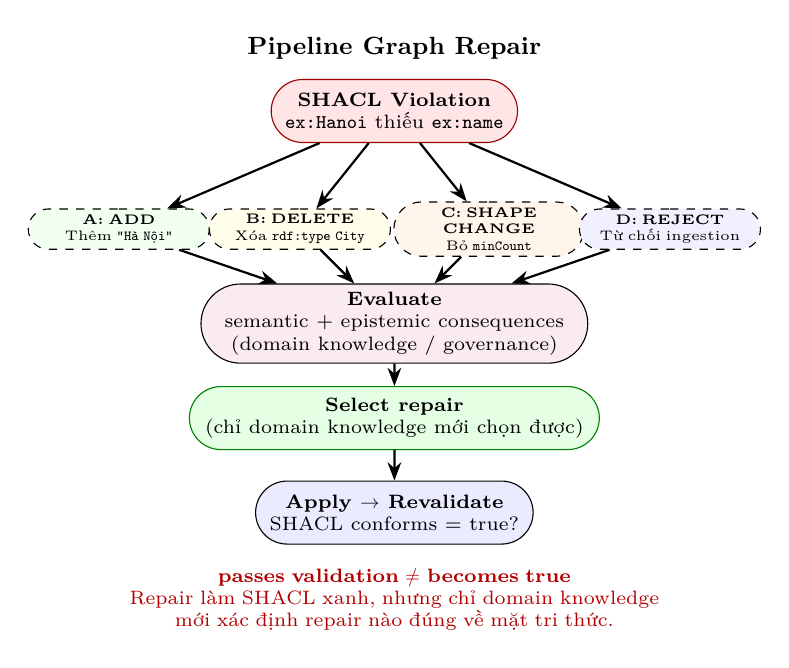
\begin{tikzpicture}[
  stepbox/.style={rounded rectangle,draw,minimum width=3.0cm,minimum height=0.8cm,
                  font=\scriptsize,align=center,inner sep=3pt},
  candidate/.style={rounded rectangle,draw,dashed,font=\tiny,inner sep=2pt,
                    minimum width=2.2cm,align=center,text width=2.0cm},
  arr/.style={->,>=Stealth,thick},
  title/.style={font=\small\bfseries},
]

% Title
\node[title] at (0,4.5) {Pipeline Graph Repair};

% Step 1: Violation
\node[stepbox,fill=red!10,draw=red!60!black] (violation) at (0,3.7)
  {\textbf{SHACL Violation}\\
   \texttt{ex:Hanoi} thiếu \texttt{ex:name}};

% Step 2: Candidate repairs (fan out)
\node[candidate,fill=green!6] (cA) at (-3.5,2.2)
  {\textbf{A: ADD}\\
   Thêm \texttt{"Hà Nội"}};
\node[candidate,fill=yellow!8] (cB) at (-1.2,2.2)
  {\textbf{B: DELETE}\\
   Xóa \texttt{rdf:type City}};
\node[candidate,fill=orange!8] (cC) at (1.2,2.2)
  {\textbf{C: SHAPE CHANGE}\\
   Bỏ \texttt{minCount}};
\node[candidate,fill=blue!6] (cD) at (3.5,2.2)
  {\textbf{D: REJECT}\\
   Từ chối ingestion};

% Fan-out arrows
\draw[arr] (violation) -- (cA);
\draw[arr] (violation) -- (cB);
\draw[arr] (violation) -- (cC);
\draw[arr] (violation) -- (cD);

% Step 3: Evaluate
\node[stepbox,fill=purple!8] (evaluate) at (0,1.0)
  {\textbf{Evaluate}\\
   semantic + epistemic consequences\\
   (domain knowledge / governance)};

% Fan-in arrows
\draw[arr] (cA) -- (evaluate);
\draw[arr] (cB) -- (evaluate);
\draw[arr] (cC) -- (evaluate);
\draw[arr] (cD) -- (evaluate);

% Step 4: Select
\node[stepbox,fill=green!10,draw=green!50!black] (select) at (0,-0.2)
  {\textbf{Select repair}\\
   (chỉ domain knowledge mới chọn được)};

\draw[arr] (evaluate) -- (select);

% Step 5: Apply + Revalidate
\node[stepbox,fill=blue!8] (revalidate) at (0,-1.4)
  {\textbf{Apply $\to$ Revalidate}\\
   SHACL conforms = true?};

\draw[arr] (select) -- (revalidate);

% Key warning
\node[font=\scriptsize,text=red!70!black,align=center,text width=7cm] at (0,-2.5)
  {\textbf{passes validation $\neq$ becomes true}\\
   Repair làm SHACL xanh, nhưng chỉ domain knowledge\\
   mới xác định repair nào đúng về mặt tri thức.};

\end{tikzpicture}
\end{document}
